%%%%%%%%%%%%%%%%%%%%%%%%%%%%%%%%%%%%%%%%%%%%%%
%                insertmeeting
% 1) Title (something creative & funny?)
% 2) Date (MM/DD/YYYY)
% 3) Location (ex. Hagerty High School)
% 4) People/Committees Present 
% 5) Picture 
% 6) Start Time & Stop Time (ex. 12:30AM to 4:30PM)
%%%%%%%%%%%%%%%%%%%%%%%%%%%%%%%%%%%%%%%%%%%%%%
\insertmeeting 
	{(Almost) Last Minute Prep} 
	{02/02/22} 
	{Hagerty High School}
	{Annika, Clayton, Falon, James, Jensen, Nathan, Ritam, Samantha}
	{Images/RobotPics/robot.jpg}
	{2:30 - 4:30}
	
\hhscommittee{Hardware}
\noindent\hfil\rule{\textwidth}{.4pt}\hfil
\subsubsection*{Goals}
\begin{itemize}
    \item The goal of the meeting was to fix our autonomous and ensure it works with road runner as well as design and cad a driver station for Leagues.   

\end{itemize} 

\noindent\hfil\rule{\textwidth}{.4pt}\hfil

\subsubsection*{Accomplishments}
Today, we created drawings of what we wanted our driver station to look like. In general, we wanted a place to put our controllers, the REV Driver Station, a spare REV screwdriver and finally we wanted to be able to cable manage the wires. To place the controllers, we decided on a plate with two large holes on the sides for the grips. This means that the controllers will be laying with the wire pointing towards the center of the station. For the REV Driver Station, we put a hole on the back so we can change out the battery and two holes which match the 3m screw mounts on the back. This allows us to successfully mount the REV Driver Station on the piece without any hassle. Then, we decided we wanted to manage the controller cables. To do this we mounted two 3d printed poles which we will use to make a figure eight with the wires. This prevents snagging and stress on the wires. Finally, we decided we would use Dual locks and magnets to keep the controllers on the station until we need to remove them. Before we cut the station out of Acrylic, we decided to cut it in wood. This was very eye opening as it allowed us to fix any issues which there were a couple. Firstly, the holes for the controller grips were very far off from the actual size. The actual size is about four inches long and the original design had it as 2.5 inches. Next was the width of the holes for the grips which was two inches when it needed to be around 2.5 inches. Then finally, we realized that we needed a way to prevent the controllers from being unplugged. To prevent this, we added holes for zip ties which means when force is applied to the cord, it will be prevented from being unplugged because the force will be absorbed by the connection to the Acrylic.



\hhscommittee{Multimedia}
\noindent\hfil\rule{\textwidth}{.4pt}\hfil
\subsubsection*{Goals}
\begin{itemize}
    \item Complete the Promote Video. 

\end{itemize} 

\noindent\hfil\rule{\textwidth}{.4pt}\hfil

\subsubsection*{Accomplishments}
Today, we submitted all of the completed scenes into the Google Drive folder and replaced images with their updated versions. Then, we worked on replacing old images with ones already put into the iMovie that we were dissatisfied with. The audio for the VoiceOver had been recorded already and was put into the file along with the song we had chosen, and all that was left today was to put all the remaining aspects together, like the completed ended card. Afterwards, we uploaded the video to Discord so it could be peer reviewed by our mentors and team. After getting some suggestions, we acted upon them by drawing a few more frames and editing the sound of the background music at the beginning. Then, a few hours later, we uploaded once more, and it was set to be uploaded to Youtube. Finally, the Promote video was complete!


\begin{figure}[ht]
\centering
\begin{minipage}[b]{.48\textwidth}
  \centering
  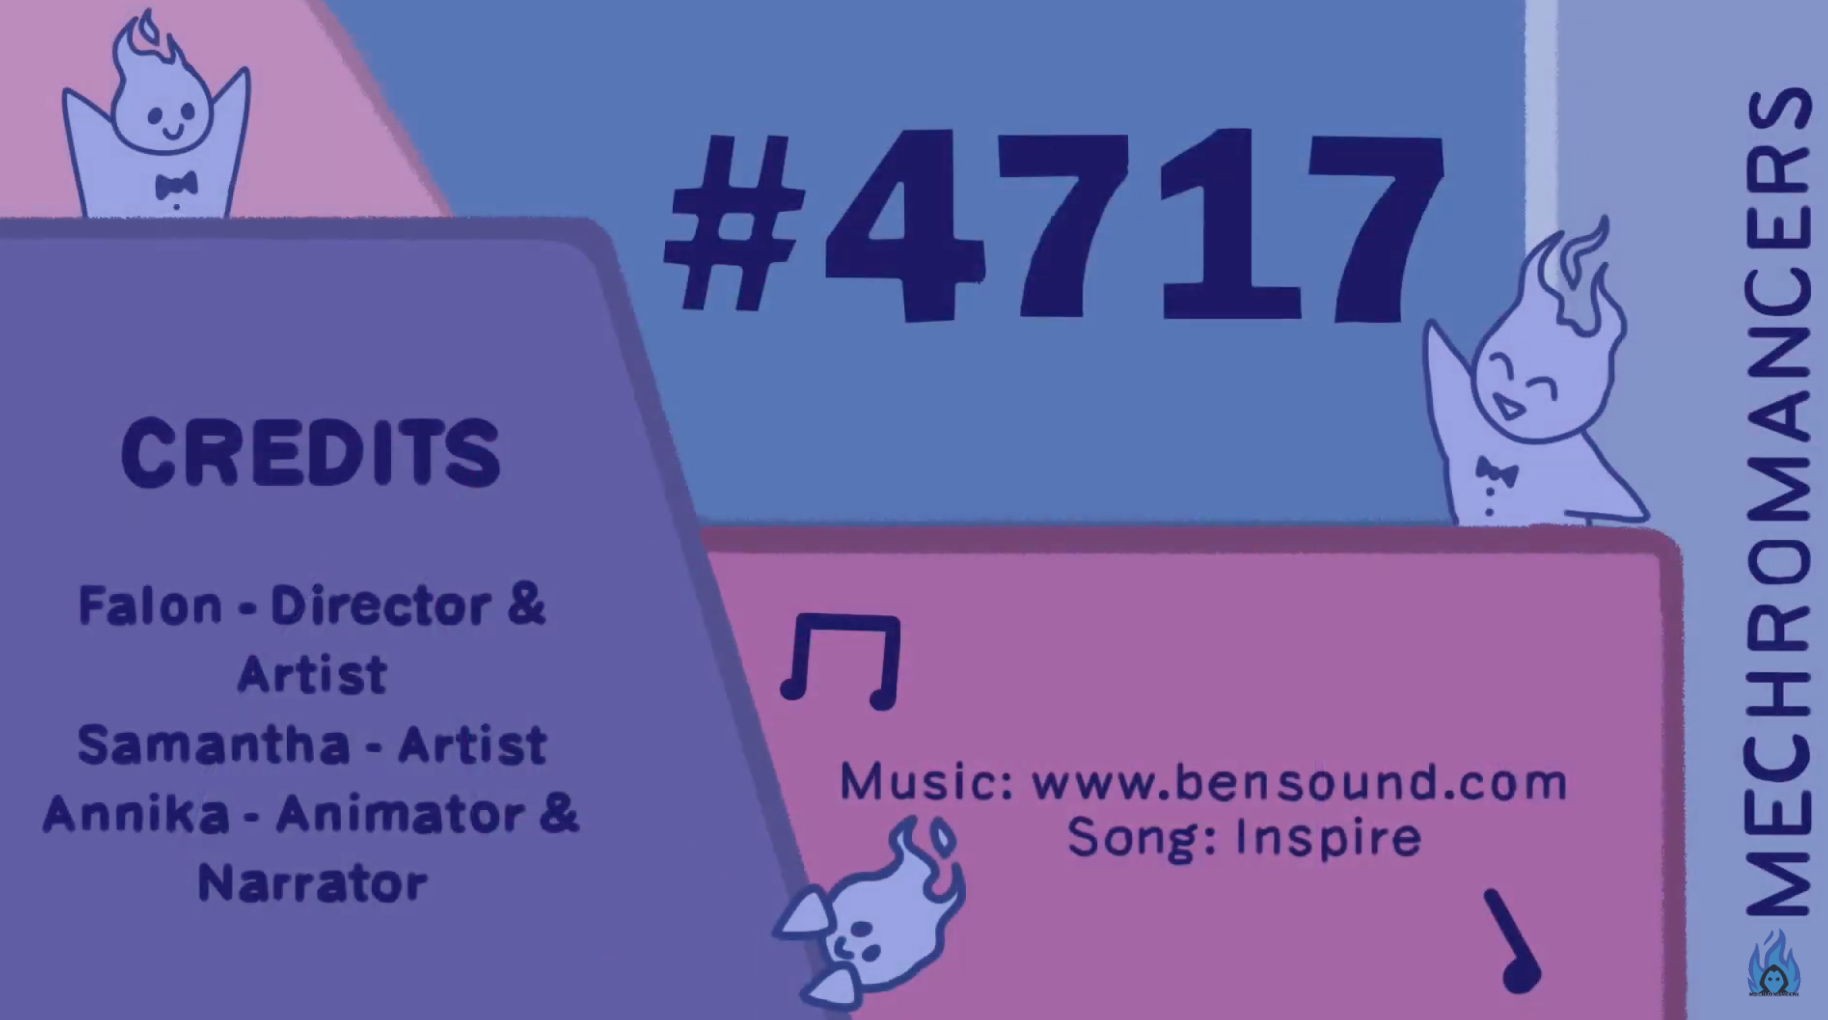
\includegraphics[width=0.95\textwidth]{Meetings/February/02-02-22/february 2___ - Falon Jones.png}
  \caption{A thumbnail idea}
  \label{fig:020222_1}
\end{minipage}%
\hfill%
\begin{minipage}[b]{.48\textwidth}
  \centering
  
\includegraphics[width=0.95\textwidth]{Meetings/February/02-02-22/idk what day - Falon Jones.png}
  \caption{Video uploaded!}
  \label{fig:020222_2}
\end{minipage}
\end{figure}


\whatsnext{
\begin{itemize}
    \item Prepare for the Space Coast League Competition.
\end{itemize} 
}

